\documentclass{article}
\usepackage{amsmath} % For math equations
\usepackage{graphicx}
\usepackage{amsfonts} % For math fonts
\usepackage{amssymb} % For math symbols
\usepackage{enumitem}
\setlist[enumerate,1]{label=\arabic*.}
\setlist[enumerate,2]{label=\alph*.,itemindent=2em}

\title{Homework 2}
\author{Asher Christian 006-150-286}
\date{2024-04-20}

\begin{document}
    \maketitle
    \section{Problem 1}
    Suppose we flip a fiar coin 100 times independently
    \begin{enumerate}
        \item What is the Probability we get 50 heads?
            Sample space = $2^{100}$ possible outcomes all equally likely.
            Of those  $\binom{100}{50}$ is the number in which 50 are heads.
            \[
                \frac{\binom{100}{50}}{2^{100}} = \frac{100!}{50!50!2^{100}} \approx 0.07958923738717877
            .\] 
        \item Let $X$ be the number of heads. What is $P(40 \le X \le 60)$?
            Same sample space as before:  $2^{100}$ However the Event space is larger
            it is
            \[
                \bigcup\limits_{40 \le i \le 60} \{X = i \}
            \] 
            Because each occurance is mutually exclusive (i.e. the space of runs where 
            heads = 50 has no intersection with the space of runs where heads = 60)
            It is enough to add the respective probabilities
            \[
                \sum_{i=40}^{60} P(X=i) = \sum_{i=40}^{60} \frac{100!}{(100-i)!i!2^{100}} \approx 0.964799799782
            \] 
        \item Let \[
        Z_i =
        \begin{cases}
            1 & \text{if the $i$-th flip is heads} \\
            0 & \text{ if the $i$-th flip is tails}
        \end{cases}
        .\]    
        Express $X$ in terms of $Z_i$.
        \[
            X = \sum_{i=0}^{100} Z_i
        .\] 
    \end{enumerate}
    \section{Problem 2}
    Draw a Galton board with 5 Layers
    \begin{figure}[htbp]
      \centering
      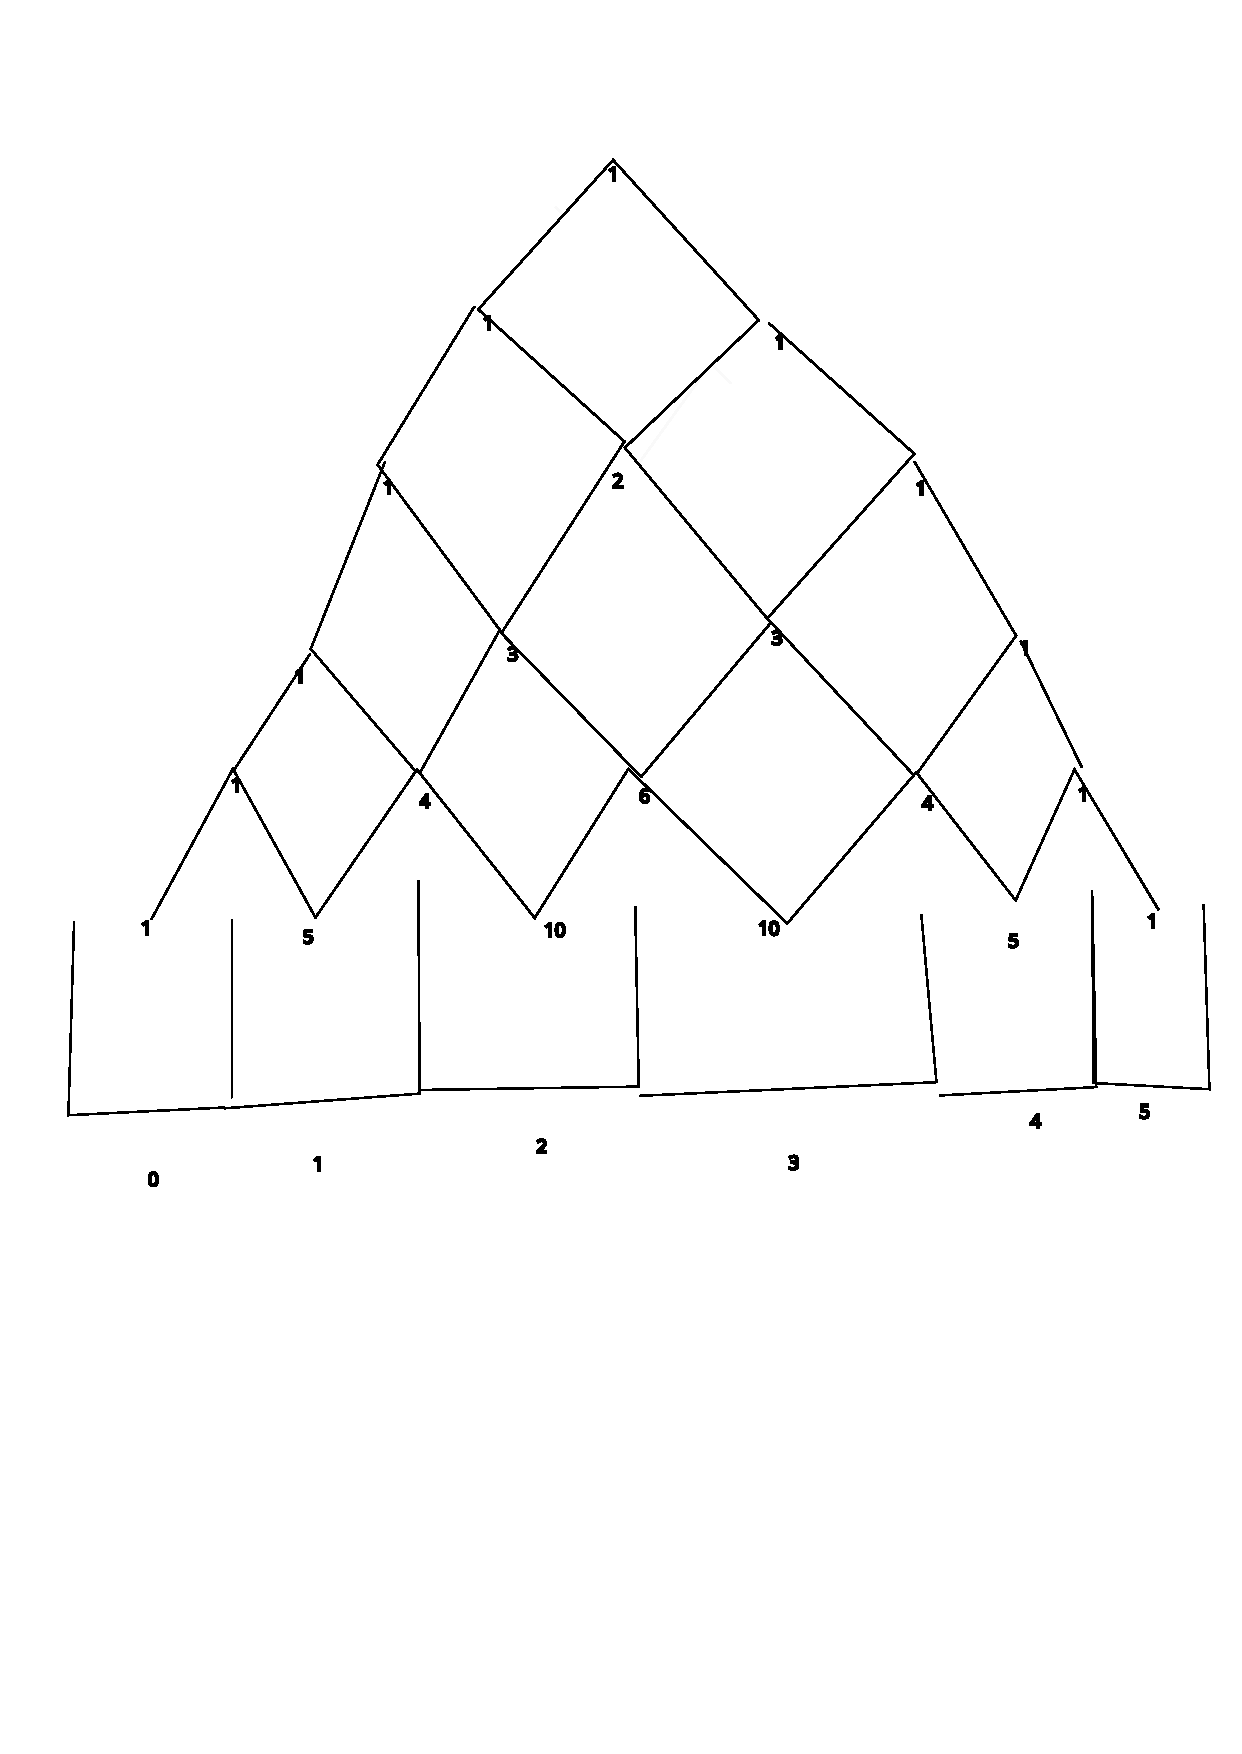
\includegraphics[width=0.8\textwidth]{designs/bitmap.pdf}
      \caption{Galton Board With Pascal's triangle overlay}
      \label{fig:example}
    \end{figure}
    \begin{enumerate}
        \item
            Draw the corresponding Pascal's triangle

        \item Suppose we label the bins by 0, 1, 2, 3, 4, 5. Calculate the probability that the ball drops
into each bin
            \[
            P(0) = \frac{1}{32}, 
            P(1) = \frac{5}{32}, 
            P(2) = \frac{10}{32}, 
            P(3) = \frac{10}{32}, 
            P(4) = \frac{5}{32}, 
            P(5) = \frac{1}{32}, 
            .\] 
        \item Suppose we drop 1 million balls. What are the proportions of balls in these bins?
            The proportions will correspond to the above results. Most balls will land in the second
            and third buckets with slightly less in the 1st and 4th and very few in the 0th and 5th buckets.

    \end{enumerate}
    \section{Problem 3}
    Random walk of integers with $X_0=0$ $X_{t+1} = X_t + \epsilon_t$\[
    \epsilon_t = 
   \begin{cases}
       1 & P = \frac{1}{2} \\
       -1 & P = \frac{1}{2}
   \end{cases}
    .\] 
    \begin{enumerate}
        \item At time $t=5$, what are the possible values for $X_t$?
            $X \in \{-5,-3,-1,1,3,5\}$
        \item What is the probability of each value in (1)?
             \[
            P(-5) = \frac{1}{32},
            P(-3) = \frac{5}{32},
            P(-1) = \frac{10}{32},
            P(1) = \frac{10}{32},
            P(3) = \frac{5}{32},
            P(5) = \frac{1}{32},
            .\] 
        \item What is $P(X_{t+1} = j| X_t = i)$?
            \[
            P = 
            \begin{cases}
                \frac{1}{2} & |i-j| = 1 \\
                0 & |i-j| \ne 1
            \end{cases}
            .\]
        \item  Interpret (2) in terms of 1 million people doing the random walk simultaneously and inde-
            pendently, all starting from 0.
            The probabilities are equivalent to that of a 5 level galton board. Thus, the various positions of the people
            should allign with those of the galton board with large masses of people at 1 and -1 and less at 3, -3 and fewest at 5, -5
            
            
    \end{enumerate}
   \section{Problem 4}
   Write R code to simulate flipping a fair coin 100 times independently. Let X be the
number of heads. Repeat the experiment 1000 times. Plot the histogram of these 1000 X. Also
plot the histogram of X/100.
    \begin{figure}[htbp]
      \centering
      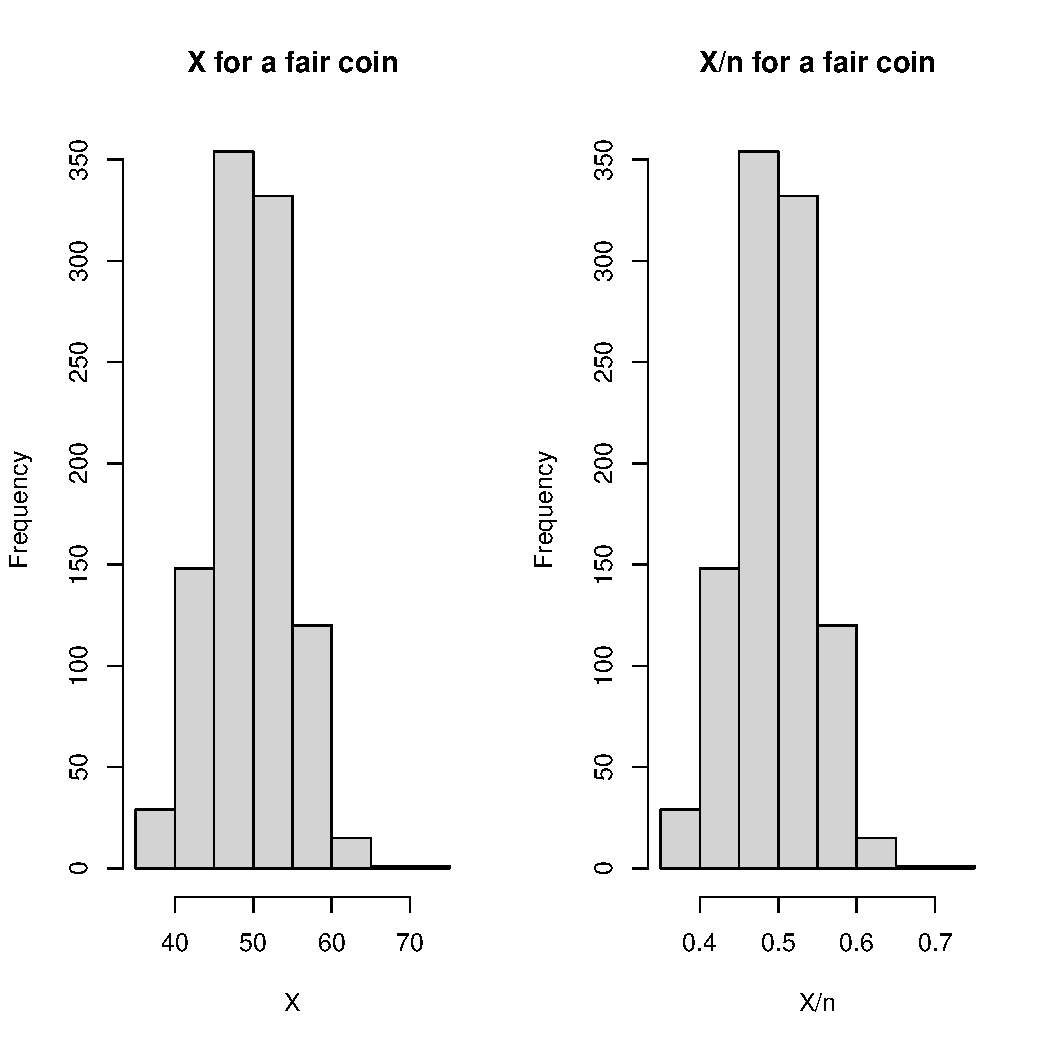
\includegraphics[width=0.8\textwidth]{fair.pdf}
      \caption{Flipping a fair coin}
      \label{fig:histogram}
    \end{figure}
    \begin{figure}[htbp]
      \centering
      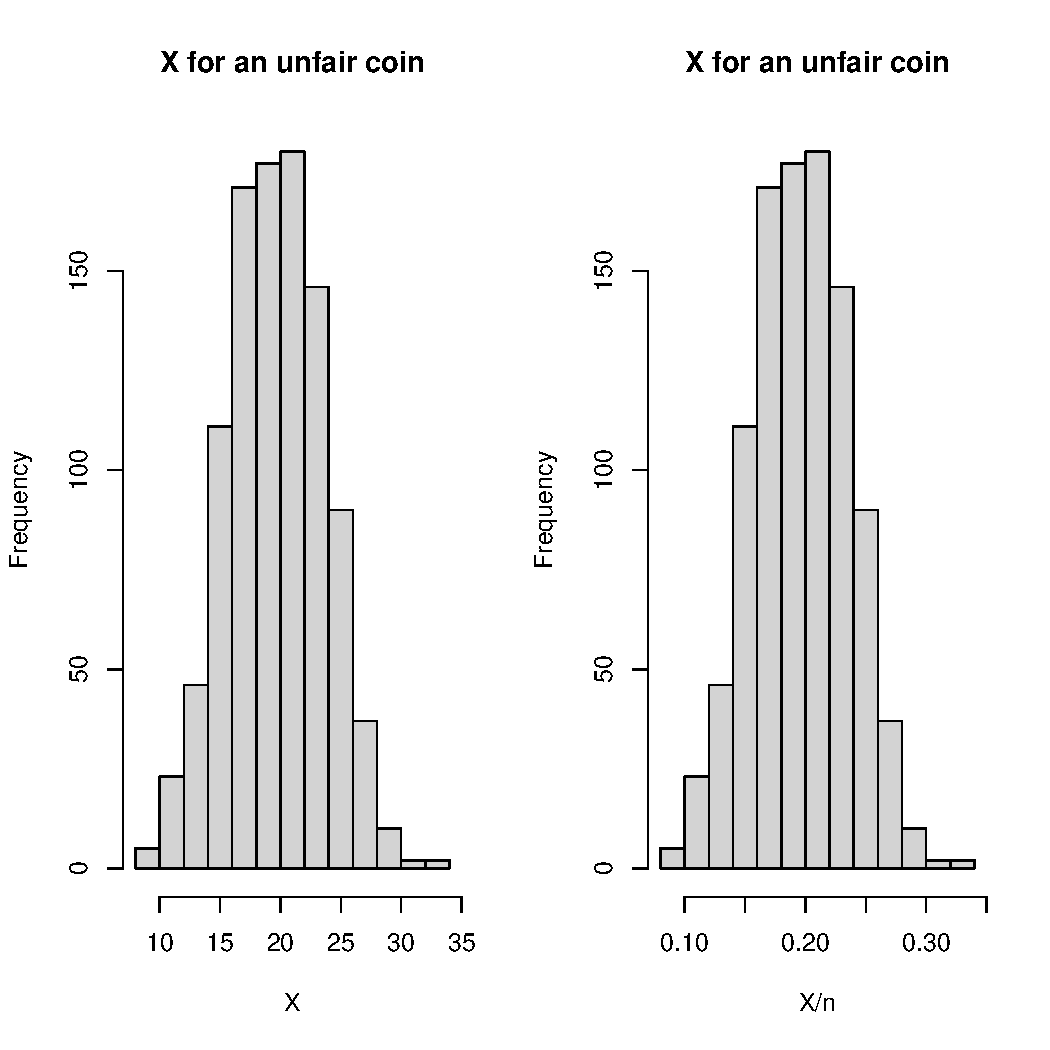
\includegraphics[width=0.8\textwidth]{unfair.pdf}
      \caption{Flipping an unfair coin}
      \label{fig:histogram}
    \end{figure}


\end{document}
